\begin{figure}[t]
\centering
\begin{subfigure}{.5\textwidth}
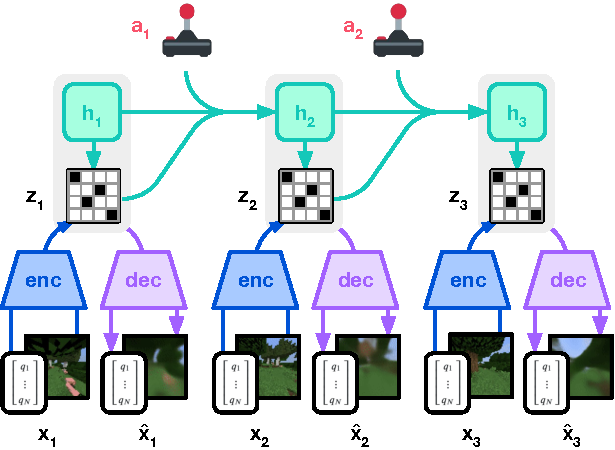
\includegraphics[width=\linewidth]{model/model_wm}
\caption{World Model Learning}
\end{subfigure}\hfill%
\begin{subfigure}{.43\textwidth}
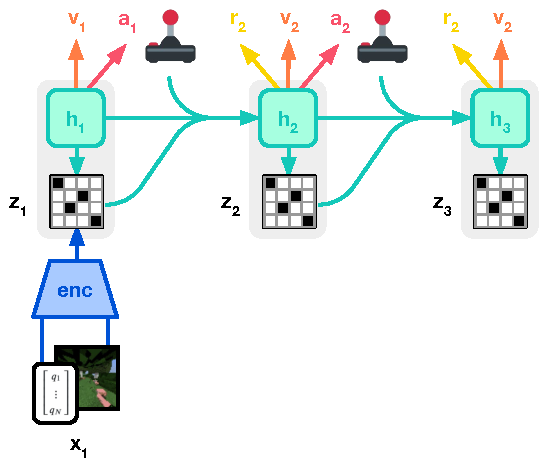
\includegraphics[width=\linewidth]{model/model_ac}
\caption{Actor Critic Learning}
\end{subfigure}
\caption{Training process of DreamerV3. The world model encodes sensory inputs into a discrete representation $z_t$ that is predicted by a sequence model with recurrent state $h_t$ given actions $a_t$. The inputs are reconstructed as learning signal to shape the representations. The actor and critic learn from trajectories of abstract representations predicted by the world model.}
\label{fig:model}
\end{figure}